\documentclass[a5paper,12pt]{article}
\usepackage{xeCJK}
\usepackage{fontspec}
\usepackage[top=-10mm,left=10mm,bottom=30mm,right=10mm]{geometry}
\usepackage{multicol}
\usepackage{setspace}
\usepackage{wrapfig}
\usepackage{xcolor}
\usepackage{graphicx}
\usepackage[backend=biber,style=mla]{biblatex}

\pagestyle{empty}
\addbibresource{hcl}

\definecolor{blue}{rgb}{0.2,0.15,0.1}
\definecolor{deepblue}{rgb}{0.4,0.3,0.2}
\graphicspath{{./images/}}

\setmainfont{TimesNewerRoman}
\setCJKmainfont{AsebiMin}

\newcommand{\CJKnumber}[1]{{#1}}
\newcommand{\explain}[2]{{$\bullet$}〔{#1}〕{#2}}
\newcommand{\go}[2]{\\{$\bullet$}請考\textcolor{blue}{#2}。 }
\newcommand{\entry}[4]{{\par{{\vspace{1.5mm}{\textcolor{deepblue}{#1}}{\textsuperscript{\CJKnumber{#2}}}{#3}}}}}
\newcommand{\also}[1]{\\亦曰\textcolor{blue}{#1}。}
\newcommand{\samp}[2]{{#1}曰:『{#2}』}
\newcommand{\syn}[2]{通\textcolor{blue}{#1}\textsuperscript{\CJKnumber{#2}}。}
\newcommand{\ant}[2]{對\textcolor{blue}{#1}\textsuperscript{\CJKnumber{#2}}。}

\begin{document}
\linespread{1.25}
\begin{wrapfigure}{r}{60mm}
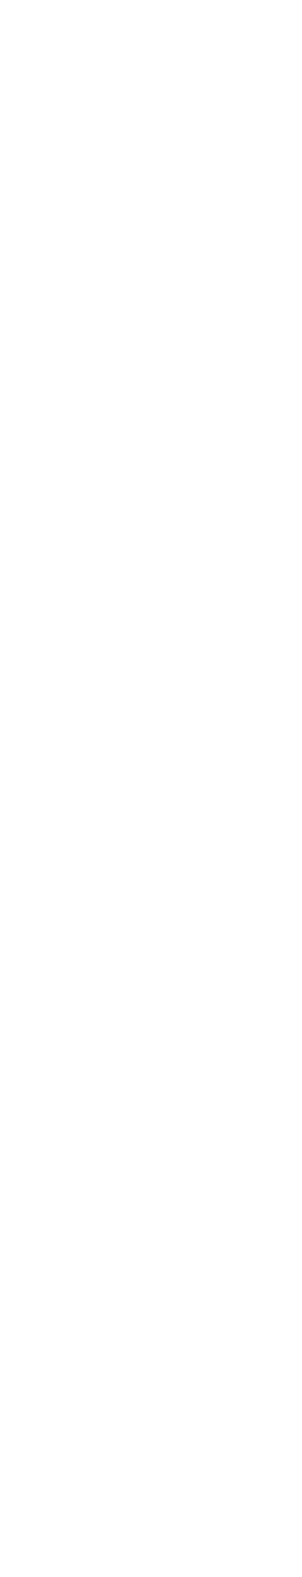
\includegraphics[height=220mm]{cover.png}
\end{wrapfigure}
\hfill
\vfill
{\fontsize{32}{32}\textcolor{deepblue}{漢詞林}}\\
{\textcolor{blue}{李世鎬}\hspace{14pt}編著}
\vspace{64pt}
\newpage
\addtolength{\topmargin}{20mm}
\linespread{1.25}
\section{序}
華夏、雞林、扶桑之類、古以漢文爲國風之礎矣。
古欲習漢文、以字典爲寶。
字典雖有文字之解、未有詞彙之解。
各國、雖有其辭書者、以諺解漢。
他國之人視、畫中之餅也耳。
以漢解漢、四海蒼生之習漢文者、皆可以讀。
余願此書爲江湖諸賢所補、爲四海諸學所寶耳。
\section{範例}
此書之範例如左。
\par 第一條:「各項、取諸漢文古典、順之若康熙字典。」
\par 第二條:「諺字與邦字、載而明之。」
\par 第三條:「詞之常同而綴之者、亦載之矣。」
\par 第四修:「變品之事、若從常道、不之載。」


\section{詞典}
\input{hcl-entries.tex}

\appendix
\printbibliography

\end{document}
